\section{Înțelegerea imaginilor}

Așa cum am precizat mai devreme, înțelegerea conținutului bonurilor fiscale din imagini reprezintă principala provocare a acestui proiect. În mod natural, această funcționalitate se desparte în două sarcini:

\begin{itemize}
  \item 
  Recunoașterea textului;
  \item
  Extragerea informațiilor din textul neprocesat;
\end{itemize}

Metode mai bune pentru a rezolva această provocare pot ține cont de imagini și pentru a doua sarcină și pot folosi metode mai avansate, de \emph{machine learning}, odată cu colectarea mai multor date. De aceea am implementat funcționalitatea de colectare de date, care va fi discutată într-o secțiune viitoare. Aceste opțiuni sunt subiectul unor cercetări viitoare.

\subsection{Recunoașterea textului}

O necesitate pentru rezolvarea acestei sarcini este aceea ca procesarea să se facă pe dispozitiv. Astfel, datele utilizatorului nu părăsesc dispozitivul decât cu acordul său.

O soluție \emph{open source} populară pentru rezolvarea problemelor OCR este \emph{Tesseract} \cite{Tesseract}. Pentru dezvoltatorii de aplicații mobile, Google oferă librăria \emph{Firebase Vision}, cu suport gratuit pentru OCR pe dispozitiv. Comparația dintre cele două soluții a fost făcută astfel:

\begin{itemize}
  \item 
  Firebase Vision a fost rulat folosind un test de instrumentare, întrucât această librărie nu poate rula decâ pe un dispozitiv mobil;
  \item
  Tesseract a fost rulat pe un computerul personal, folosind \emph{Python};
  \item
  Imaginea a fost preprocesată doar pentru Tesseract, întrucât această librărie nu oferă o performanț satisfăcătoare pe imagini neprocesate;
  \item
  Preprocesarea a constat în aplicarea unui algoritm care să elimine fundalul, să transforme imaginea î alb-negru și să uniformizeze luminozitatea;
  \item
  Asupra ambelor rezultate a fost aplicat un algoritm care să grupeze chenarele de text pe linii;
\end{itemize}

Anexa \ref{apx:Anexa1} cuprinde cele două script-uri folosite pentru comparație. Rezultatele obținute sunt prezentate în figura ... .

De menționat este și efortul necesar pentru a integra \emph{Tesseract} într-o aplicație mobilă. În același timp, \emph{Firebase Vision} este disponibilă ca o dependință \emph{gradle}.

Performanța superioară a \emph{Firebase Vision} ar fi suficientă pentru a alege această librărie. La aceasta se adaugă și ușurința integrării și lipsa necesității de preprocesare. Dezavantajul major al acestei librării este integrarea unui serviciu extern, care nu este open source în codul aplicației, dar acesta nu este unul foarte mare pentru versiunea curentă a aplicației. Așadar, pentru sarcina de OCR am ales soluția \emph{Firebase Vision}.

\subsection{Extragerea informațiilor din text}

Procesarea textului rezultat în urma procesului de OCR se face pe baza unor reguli observate în majoritatea bonurilor fiscale. Firebase Vision returnează textul și chenarele de text, grupate în blocuri, linii și elemente, în funcție de coordonatele geometrice din imagine. Această organizare pe blocuri nu este de folos în procesarea de față, dar organizarea pe linii este, din moment ce informația de pe bonurile fiscale este așezată în format cheie-valoare, pe linii. De aceea, prima etapă în extragerea informațiilor este renunțarea la structura de blocuri și organizarea în linii raportate la întregul document. Această etapă se face după algoritmul:

\begin{enumerate}
  \item
  Extrage liniile din blocuri;
  \item
  Sortează liniile de sus în jos, în funcție de punctul lor de mijloc; Consideră liniile ca fiind elementele OCR;
  \item
  Grupează elementele OCR după distanța relativă dintre punctele lor de mijloc: elementele la o distanță mai mică de jumătate din media înălțimii tuturor elementelor se află în același grup;
\end{enumerate}

Implementarea acestui algoritm se găsește în Anexa \ref{apx:Anexa2}.

Având textul din imagine organizat în grupuri de cuvinte apropiate (vechile linii returnate de \emph{Firebase Vision}) și linii raportate la întreaga imagine, ordonate de sus în jos, informațiile relevante sunt extrase după următoarele reguli:

\begin{itemize}
  \item
  \textbf{Numele comerciantului}:
  \begin{enumerate}
      \item
      Extrage prima linie. Dacă aceasta este formată dintr-o singură literă, continuă extragerea. Această regulă este motivată de faptul că multe bonuri pot conține la început un logo ce poate fi confundat cu o literă.
      \item
      Dacă linia curentă are înălțimea peste media tuturor liniilor, atunci verifică următoarea linie. Dacă și aceasta are înălțimea peste medie și mai puțin de 3 cuvinte, consideră numele comerciantului ca fiind concatenarea celor două linii. În caz contrar, consideră numele comerciantului ca fiind textul liniei curente.
  \end{enumerate}
  \item
  \textbf{Data achiziției}: aplică o serie de expresii regulate pentru a parsa date din întregul text. Dacă sunt găsite mai multe date, alege data cea mai apropiată de data curentă. Dacă nu este găsită nicio dată, consideră data curentă.
  \item
  \textbf{Produse și preț total}: Acestea sunt procesate parcurgând liniile de sus în jos și alcătuind o listă obiecte de tip cheie-valoare. Cheile sunt nume de produse sau cuvinte cheie care să marcheze prețul total, iar valorile sunt prețuri, numere fracționare. Produsele și prețurile aferente sunt considerate toate obiectele care sunt întâlnite deasupra primului obiect ce marchează totalul.
  \item
  \textbf{Categoria și moneda}: aceste valori sunt citite din setările predefinite și pot fi modificate de utilizator.
  \textbf{Categoria și moneda}: aceste valori sunt citite din setările predefinite și pot fi modificate de utilizator.
  \textbf{Categoria și moneda}: aceste valori sunt citite din setările predefinite și pot fi modificate de utilizator.
  \textbf{Categoria și moneda}: aceste valori sunt citite din setările predefinite și pot fi modificate de utilizator.
\end{itemize}

Implementarea detaliată a algoritmului de extragere a informațiilor este prezentat în Anexa \ref{apx:Apendix3}.

\subsection{Implementare}

Figura \ref{fig:scanner} prezintă ecranul de scanare, care este interfața cu utilizatorul a algoritmului de extragere a informațiilor. Acesta permite utilizatorului să obțină o imagine a bonului fiscal folosind camera telefonului sau importând-o din galerie. De asemenea, ecranul permite utilizatorului activarea sau dezactivarea blitz-ului. Odată ce utilizatorul atinge ecranul sau importă o imagine din galerie, este afișat un ecran de încărcare, în timp ce procesarea se face în background. La finalul procesării, utilizatorul este redirecționat către un ecran de unde poate face modificări asupra datelor extrase.

\begin{figure}[ht]
  \centering
  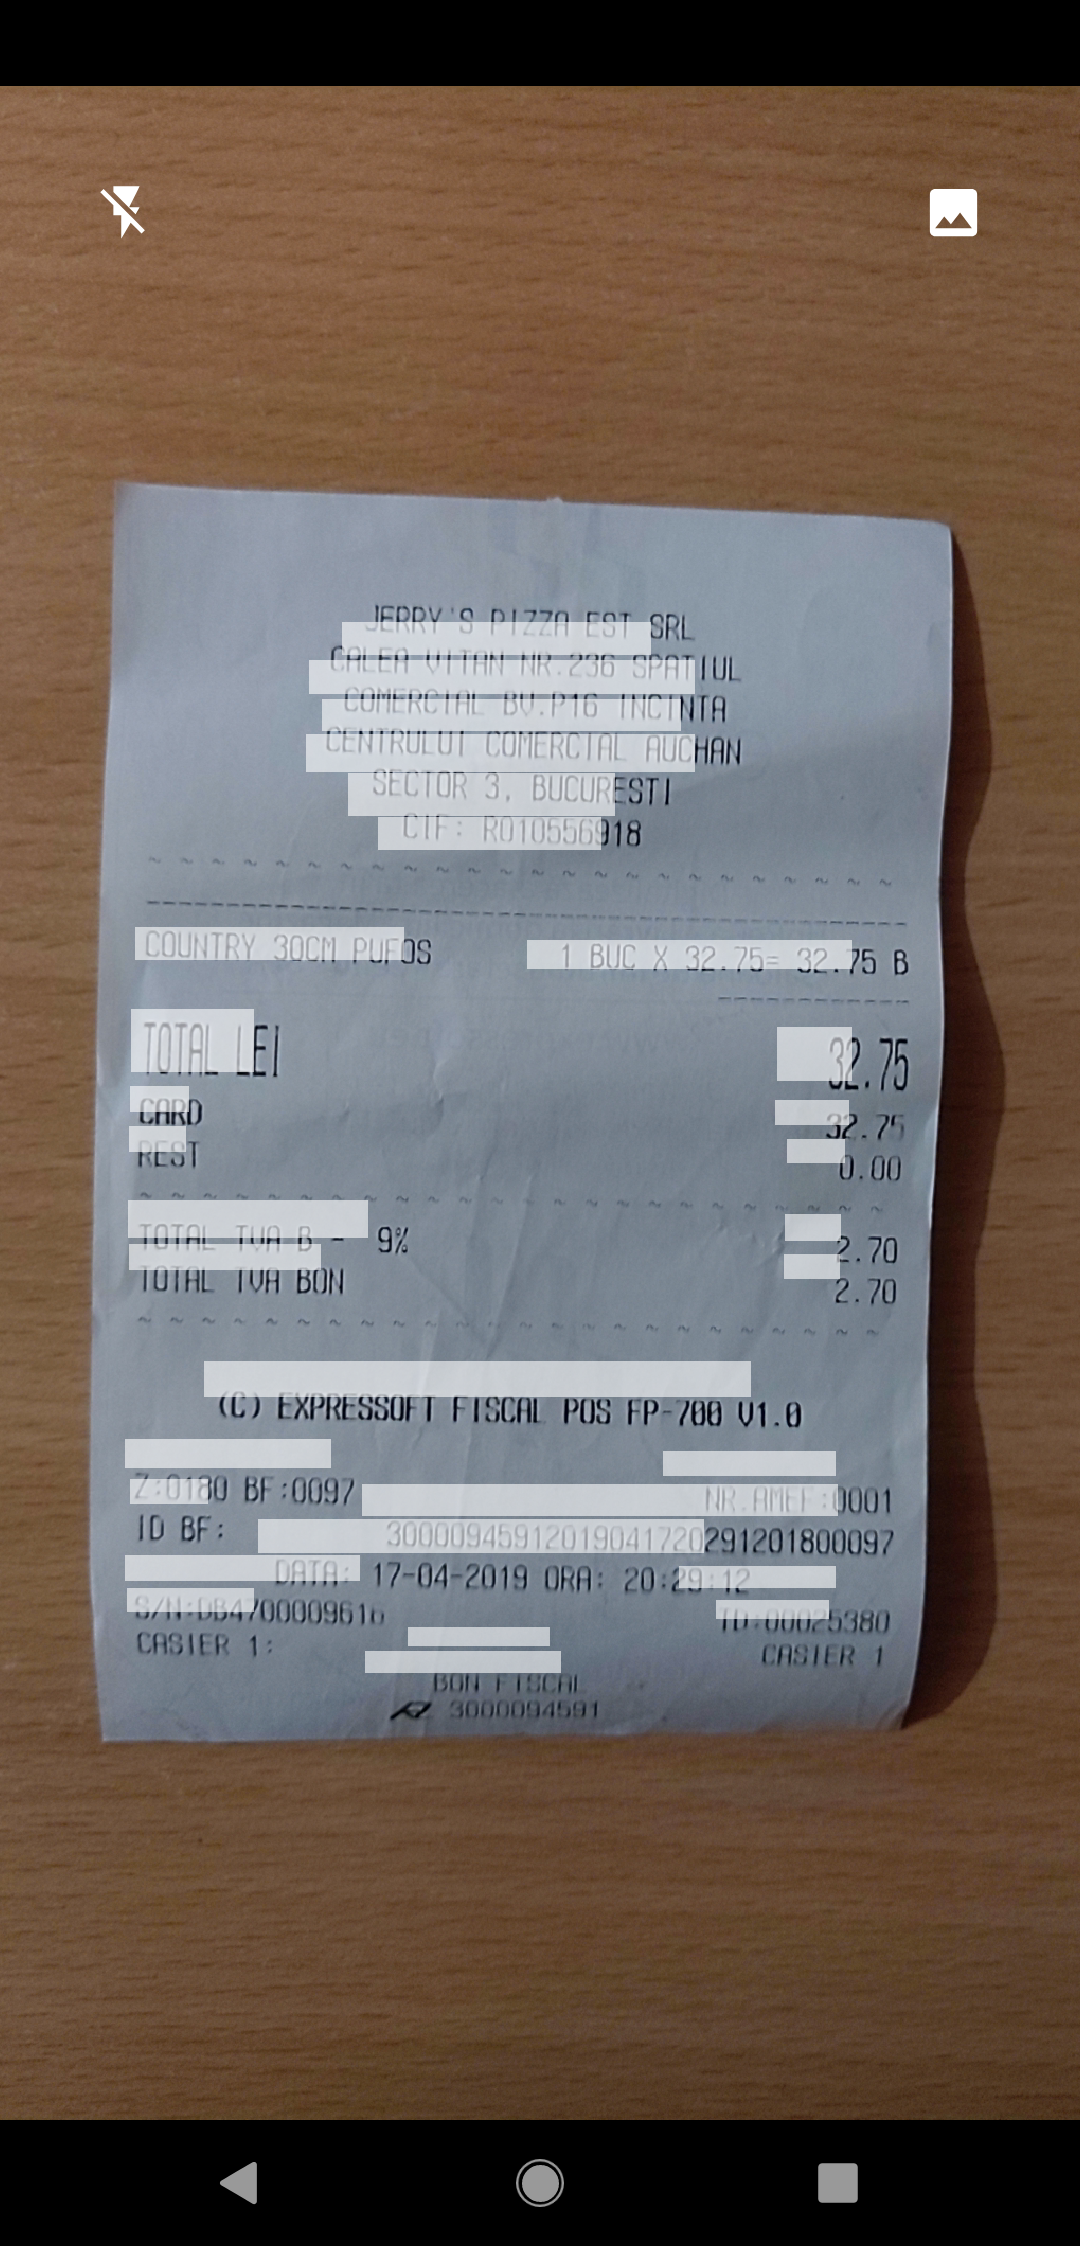
\includegraphics[width=\screenwidth]{Scanner.png}
  \caption{Ecranul de Scanare}
  \label{fig:scanner}
\end{figure}

La nivelul domeniului, algoritmul de OCR este ascuns sub interfața \texttt{Scannable}, care este implementată la nivelul infrastructurii. Aceasta expune două metode, \texttt{ocrElements()} și \texttt{image()}, ce furnizează elementele textuale și imaginea sub abstractizarea \texttt{Observable} din RxJava.

\lstinputlisting[style=javaCodeStyle, caption=Interfețele Scannable și ExtractUseCase]{./code/ScannableExtractUseCase.kt}

\texttt{ExtractUseCase} modelează și orchestrează funcționalitățile aferente ecranului de scanare:

\begin{itemize}
  \item 
  Valoarea \texttt{preview} expune un flux de elemente OCR care să fie afișate pe ecran, deasupra camerei, pentru a ajuta utilizatorul în capturarea imaginii;

  \item
  Funcția \texttt{fetchPreview} permite livrarea unui nou cadru surprins de cameră, care să fie procesat asincron, iar rezultatul să fie livrat către \texttt{preview};

  \item
  Funcția \texttt{extract} declanșează procesarea imaginii bonului și salvarea informațiilor în baza de date, returnând id-ul entității salvate;

  \item
  Valoarea \texttt{state} marchează daca o imagine este procesată pentru extragerea unui bon sau nu, sau dacă a fost întâmpinată o eroare;
\end{itemize}

Procesarea unei imagini durează în funcție de performanțele telefonului, timp de câteva secunde. Părăsirea ecranului de scanare este permisă în acest timp deoarece obiectul \texttt{ExtractUseCase} nu este distrus odată cu obiectul vizual, ceea ce nu întrerupe procesarea.
